\documentclass[../main.tex]{subfiles}
\begin{document}

\section{Optimal Control of Pitch/Travel with Feedback (LQ)}
In this task we add feedback to the optimal controller that we developed in \cref{kap:Part2OptimalControlWithoutFeedback}. Feedback is clearly needed as¨the experimental results in \cref{kap:task_10_2_experimental_results} show that the helicopter response quickly deviates from the optimal trajectory because of pitch-offset - adding feedback could reduce or eliminate this deviation.

The results achieved in this section shows that adding feedback greatly improves performance.

\subsection{Introducing feedback}
There are many approaches to adding feedback, but in this assignment only two will be considered: linear state feedback and model predictive control.

Linear state feedback adds a new control layer below the optimization layer, the advanced control layer. This layer controls the pitch setpoint to the basic control layer based on a control law that considers the optimal trajectory and the current state of the system. If the states deviate from the optimal value the input is changed accoridn gto the pitch-control equation:
\begin{equation}\label{eq:lab3_feedback}
	u_k = u_k^* - \bm{K}^T(\bm x_k - \bm x_k^*)
\end{equation}
where $u_k^*$ and $\bm x_k^*$ are the optimal input and state trajectories predicted in the optimization layer, $u_k$ is the next input and $x_k$ is the current state. $K$ is the linear state feedback term. 

In this exercise the gain matrix $K$ is calculated as an LQ controller, see \cref{kap:task_10_3_LQ_controller} for more info about the exact implementation.

Model Predictive Control (MPC) is a completely different solution: the optimal trajectory is recalculated at every timestep. See \cref{kap:10_3_mpc} for more info about how that could be implemented here.

\subsection{LQ controller} \label{kap:task_10_3_LQ_controller}
As explained in the problem description\todo{cref}, an LQ (or linear-quadratic) controller, solves the quadratic objective function given by
\begin{equation}
    J = \sum^\infty_{i=0} \Delta x_{i+1}^\top Q \Delta x_{i+1} + \Delta u_i^\top R \Delta u_i, \quad Q \ge0, \quad R > 0
\end{equation}
for a linear model
\begin{equation}\label{eq:lab3_lin_model}
	\Delta x=A\Delta x_i + B \Delta u_i
\end{equation}
without including inequality constraints.
Here $ \Delta x = x - x^*$ and $\Delta u = u - u^*$ are deviations from the optimal trajectory.

The matrix $Q$ and the scalar $R$ are the weights of the optimalization problem. $Q$ determines how much state-deviations should be penalized, while $R$ determines how much input-deviation should be punished. This allows the designer to optimize the regulator to the specific implementation: Is it more important to have low input-deviation than state-deviation?

In this system there is only one constraint on the input; that it shall not exceed 30 degrees. Therefore a small R-value compared to Q is warranted. This will produce a regulator that tries harder to minimize state-deviation than input-deviation.

\subsection{Model Predictive Control}\label{kap:10_3_mpc}
Model Predictive Control is another way of introducing feedback to an optimal control system. In an MPC controlled system the optimal response and input is recalculated at every timestep, the input used is simply the first of the optimal input values calculated at every step.

This is a drastically different approach to the LQ-method impemented in this laboratory exercise.

\subsubsection{Modified Control Hierarchy with MPC}
Rather than introducing the Advanced Control Layer with the LQ-controller; introducing MPC would introduce the feedback to the Optimization Layer instead. The optimization layer would use the current state value and generate an optimal trajectory to the target, outputting pitch-setpoints to the Basic control layer at every timestep.

\subsection{Experimental results} \label{sec:lab3_result}
It is very clear that introducing feedback produced results much better than the ones achieved without feedback, almost regardless of the tuning of the LQR regulator. This is of course what was expected.

The group performed experiments with different values of Q and R to analyze the performance of the helicopter with different tunings.

\Cref{fig:LAB3_R_variations} shows that changing the R-value did not drastically change the response, nevertheless it was observed that a larger R-value produces greater state-offset and smaller input-offset.

\Cref{fig:LAB3_Q_variations} shows that increasing the Q-value greatly reduces the offset from the optimal and actual travel response. It was also observed that this caused oscillations in the input-values.

The experimental results are consistent with the theory of the LQ controller laid out in \cref{kap:task_10_3_LQ_controller}.

The group observed that the state never reached the optimal trajectory, even with very high Q-values. The group believes that adding integration to the LQ-regulator would eliminate the stationary- and reduce the dynamic offset. This was however not explored further.

\begin{figure}[h]
    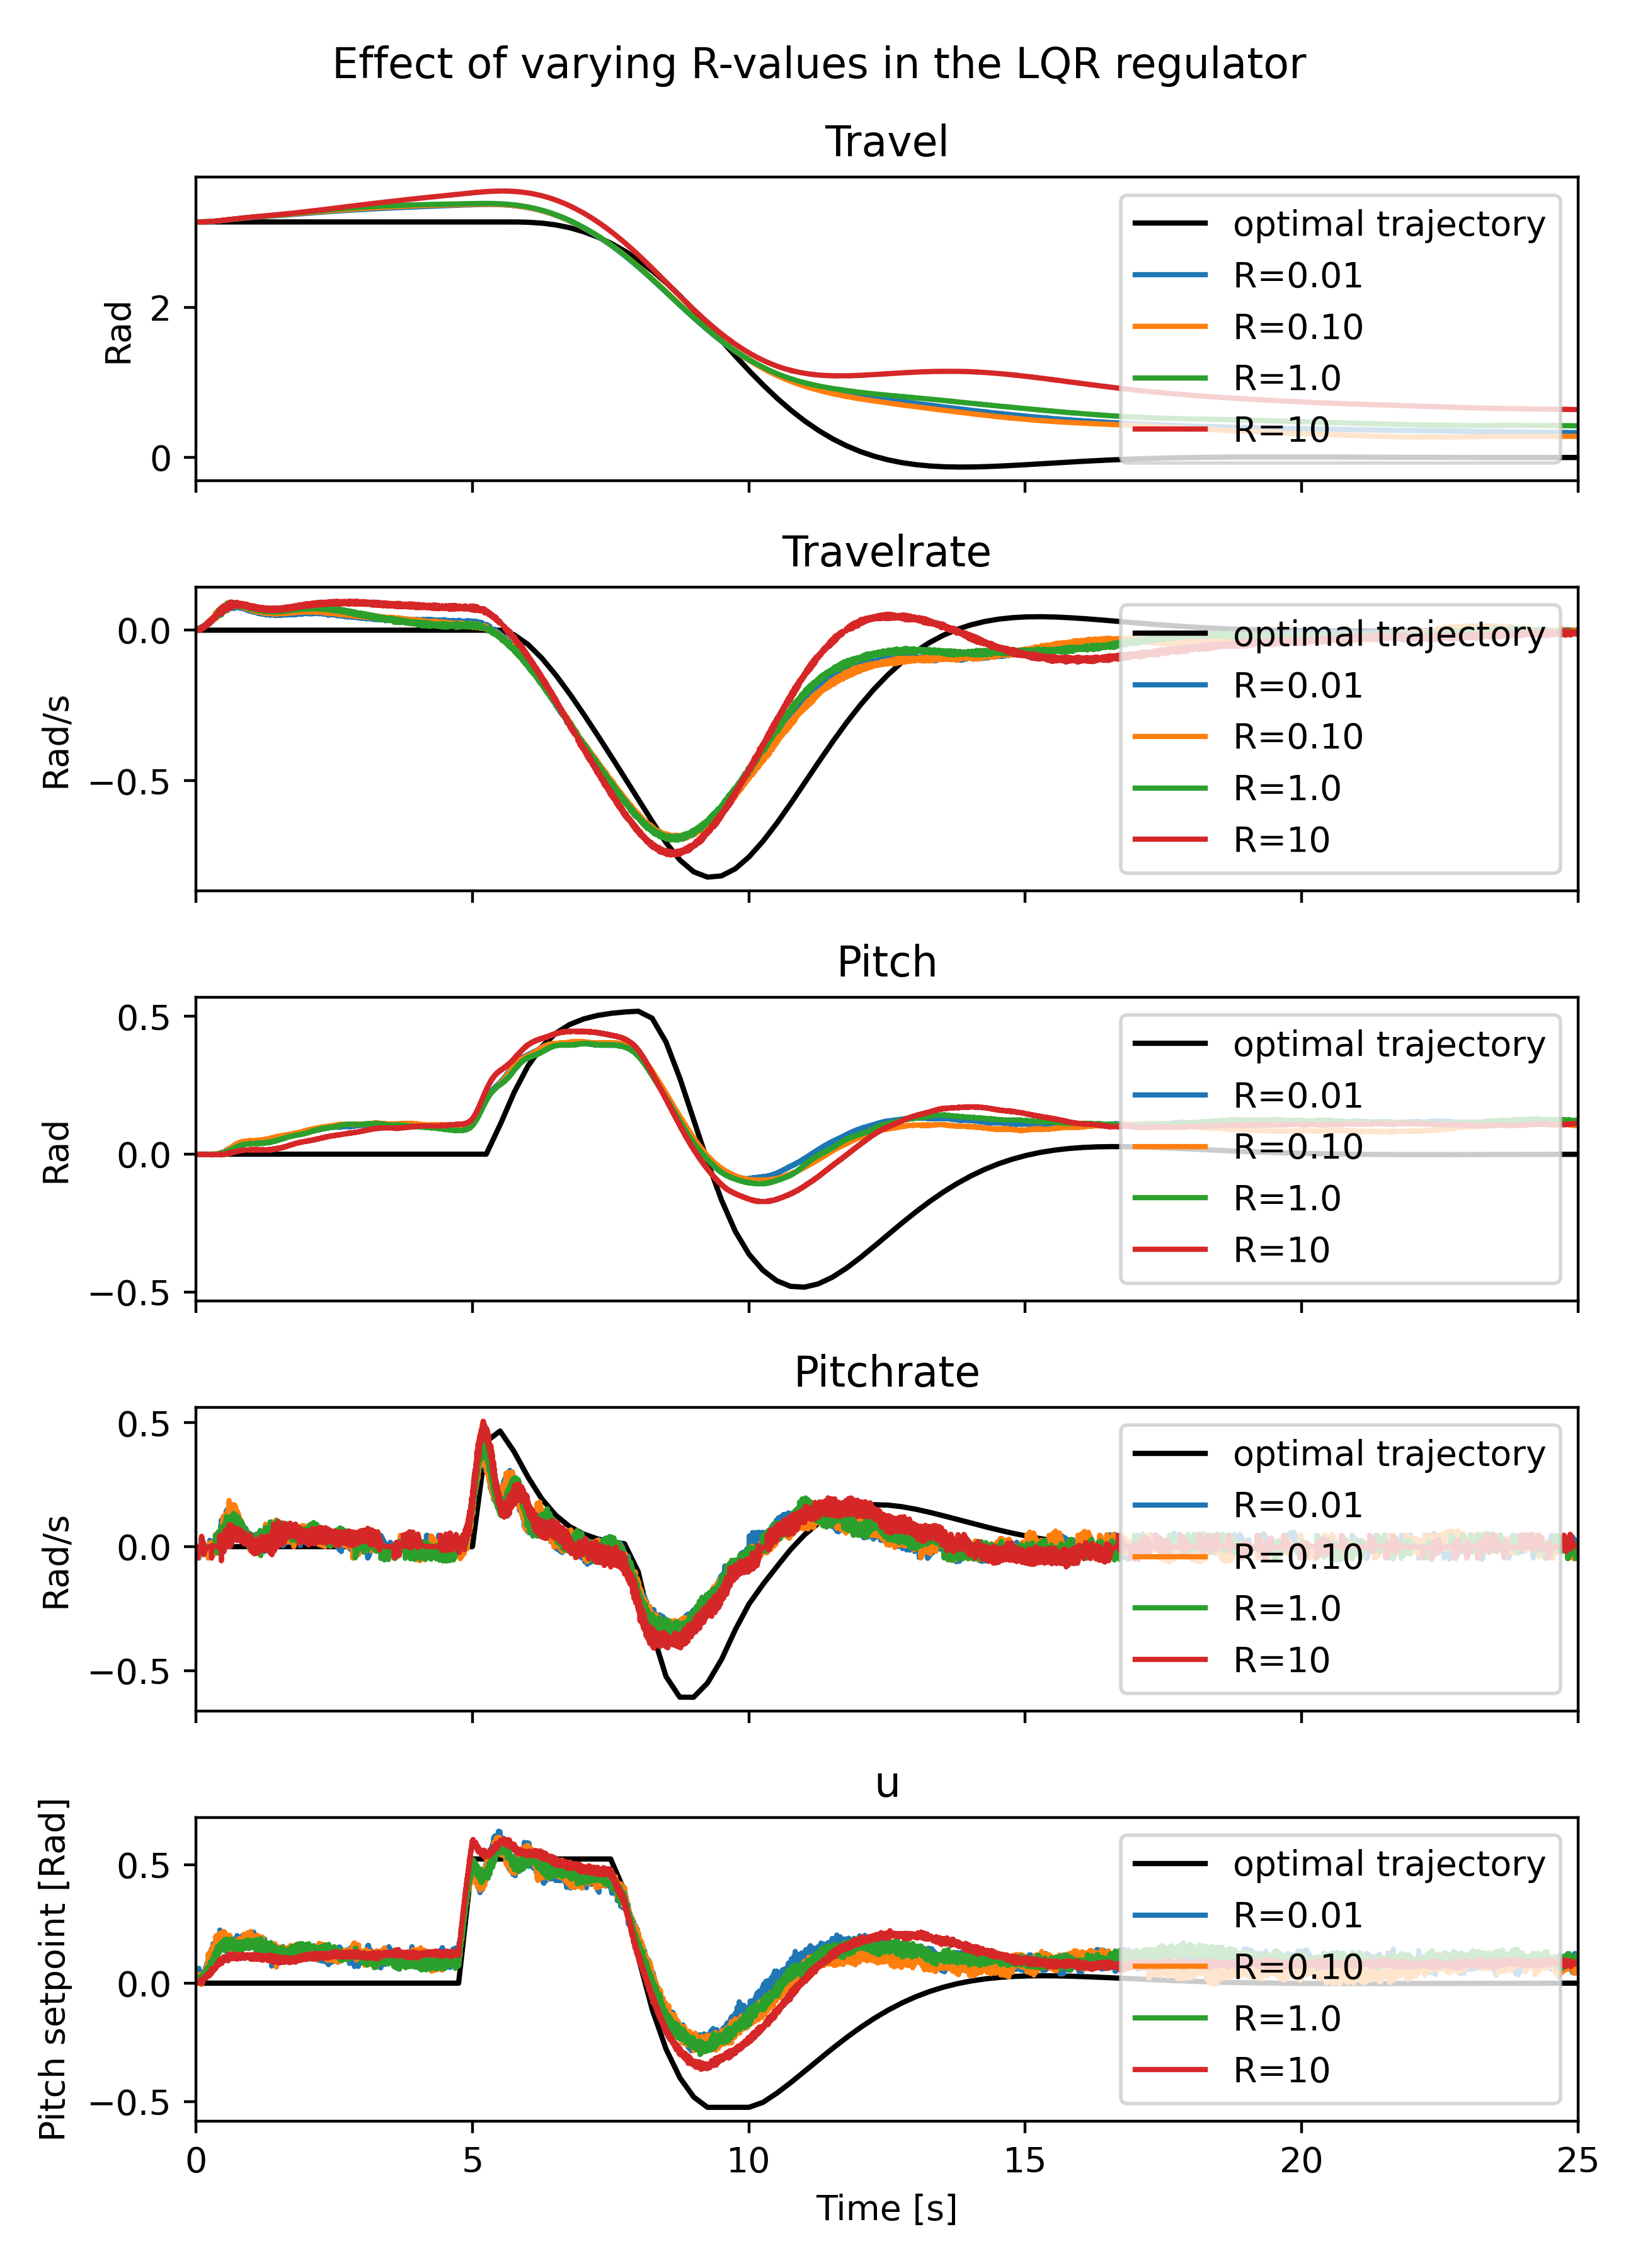
\includegraphics[width=\linewidth]{figures/LAB3_R_variations.png}
	\caption{Results of varying R-values wihle keeping Q=diag([1,1,1,1])}
	\label{fig:LAB3_R_variations}
\end{figure}

\begin{figure}[h]
	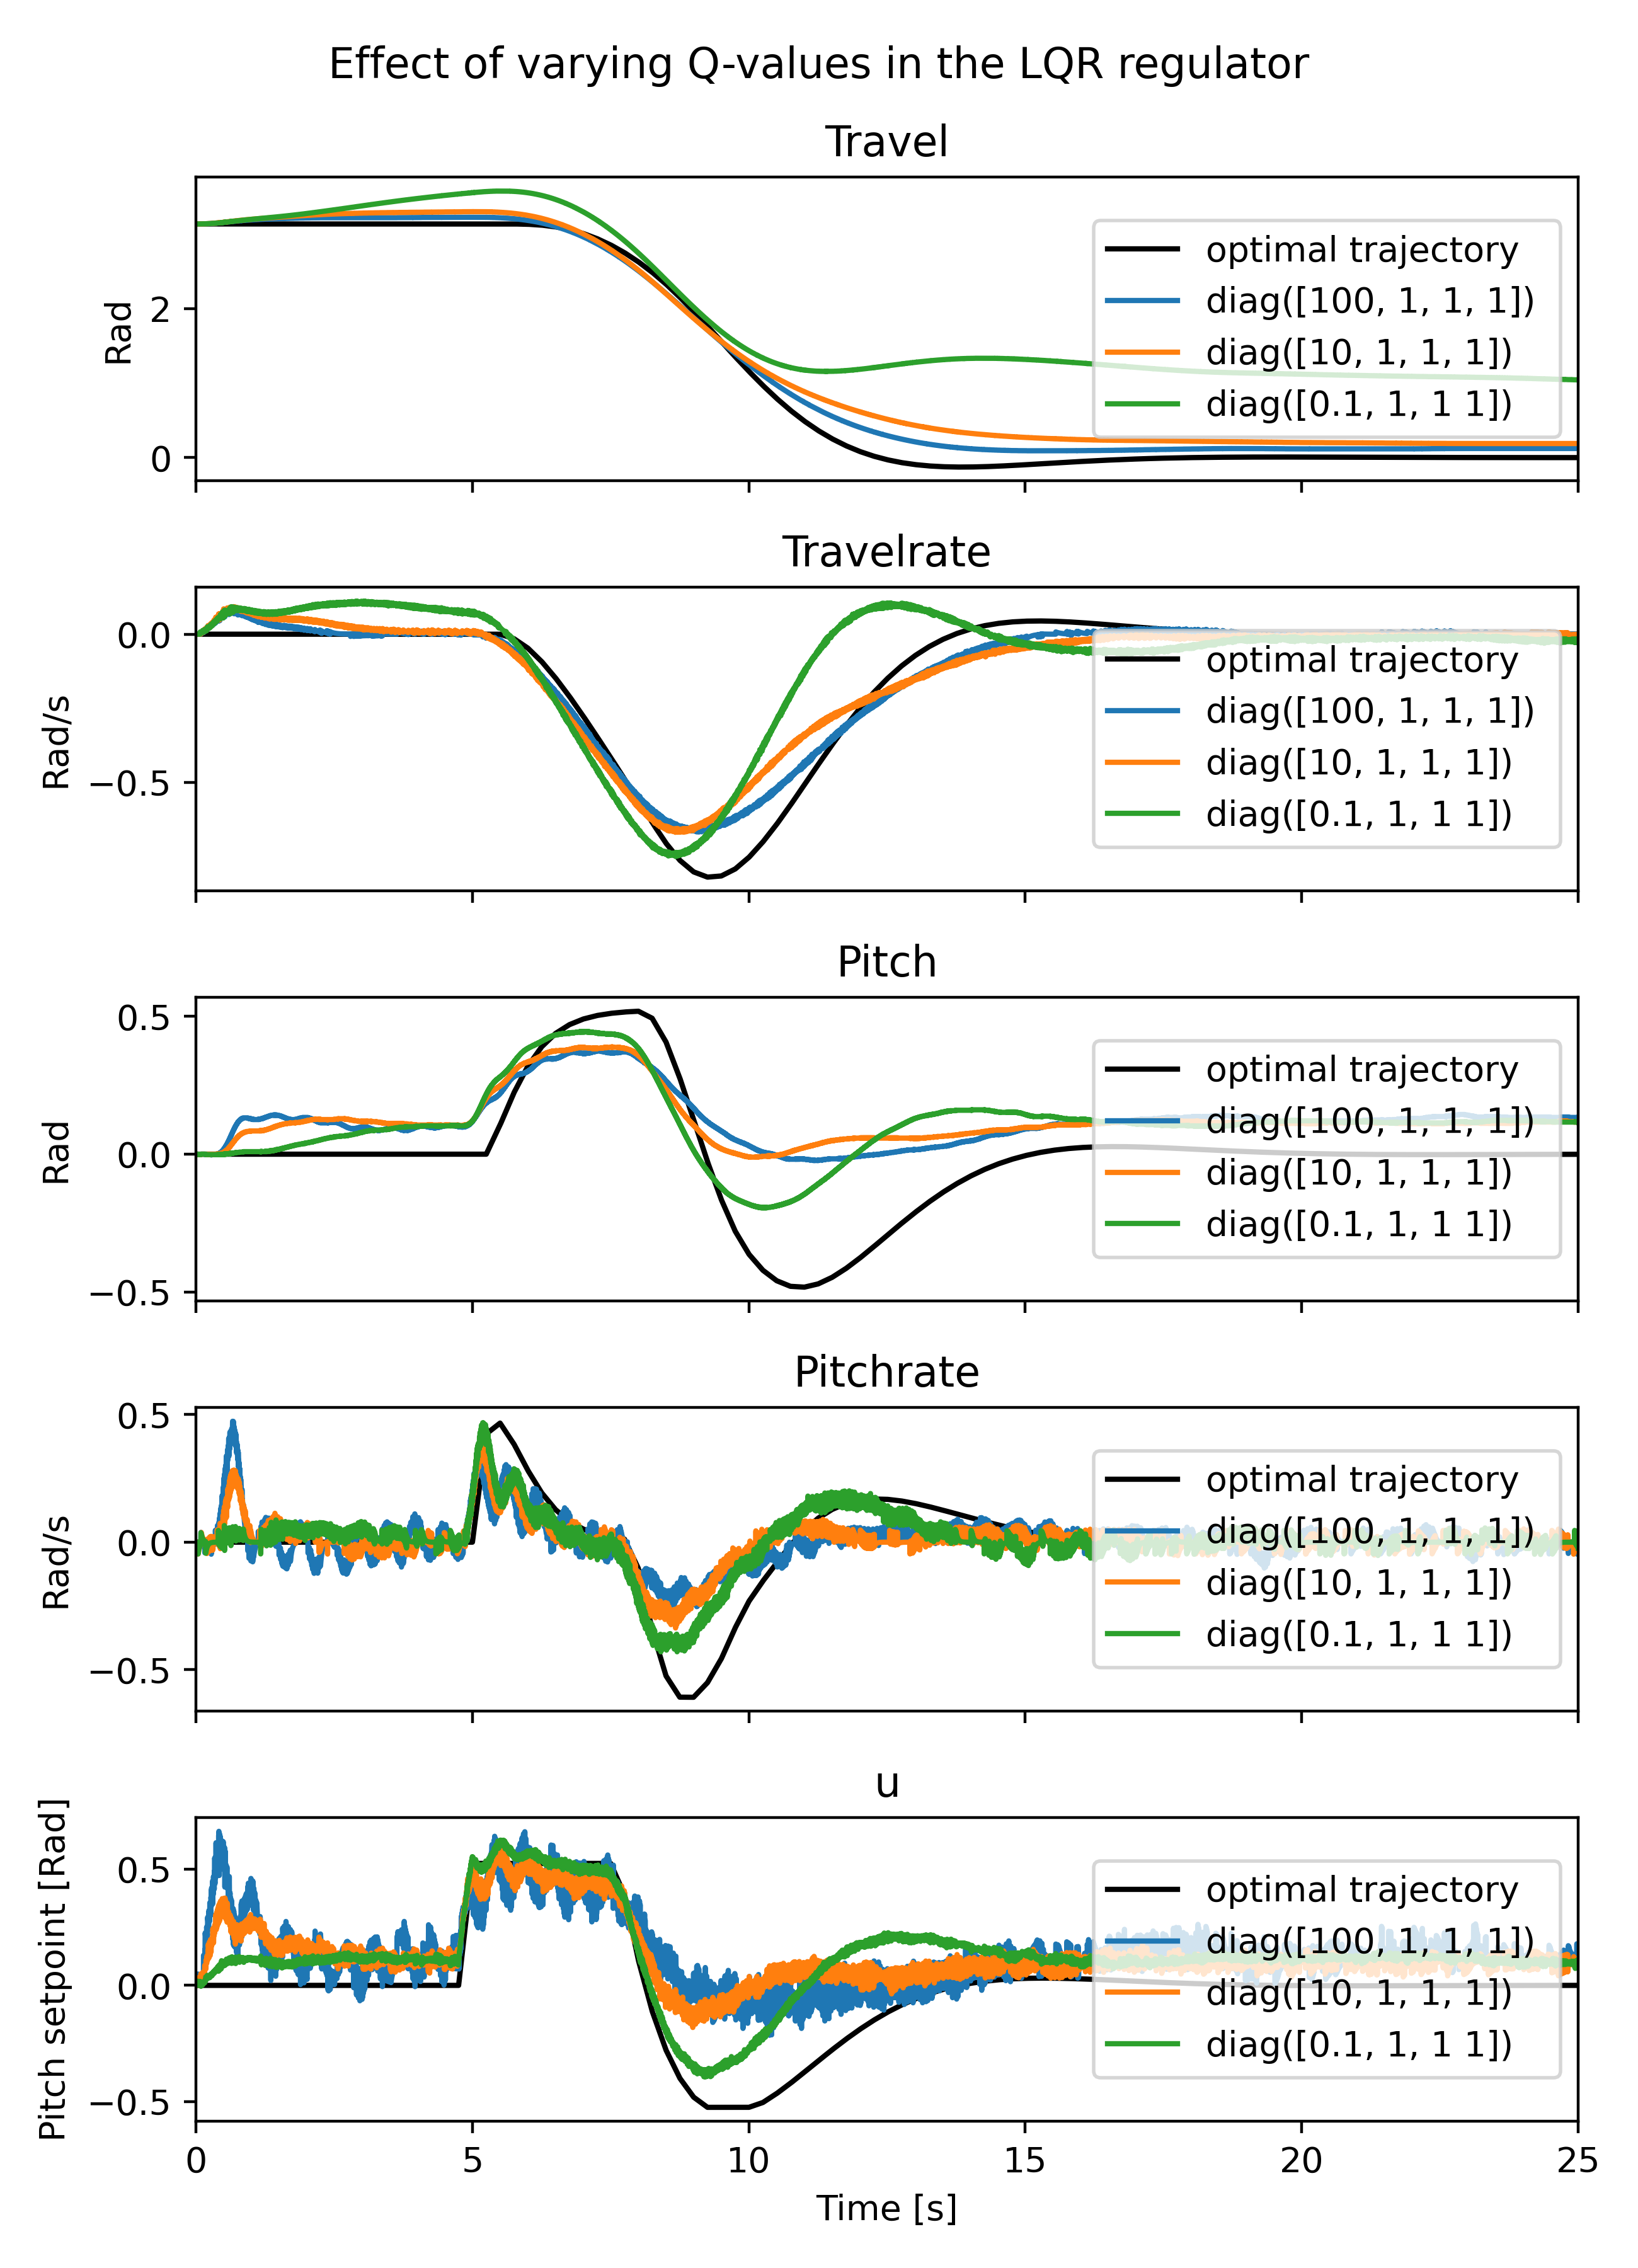
\includegraphics[width=\linewidth]{figures/LAB3_Q_variations.png}
	\caption{Results of varying Q-values while keeping $R=1$}
	\label{fig:LAB3_Q_variations_travel}
\end{figure}

\begin{figure}[h]
	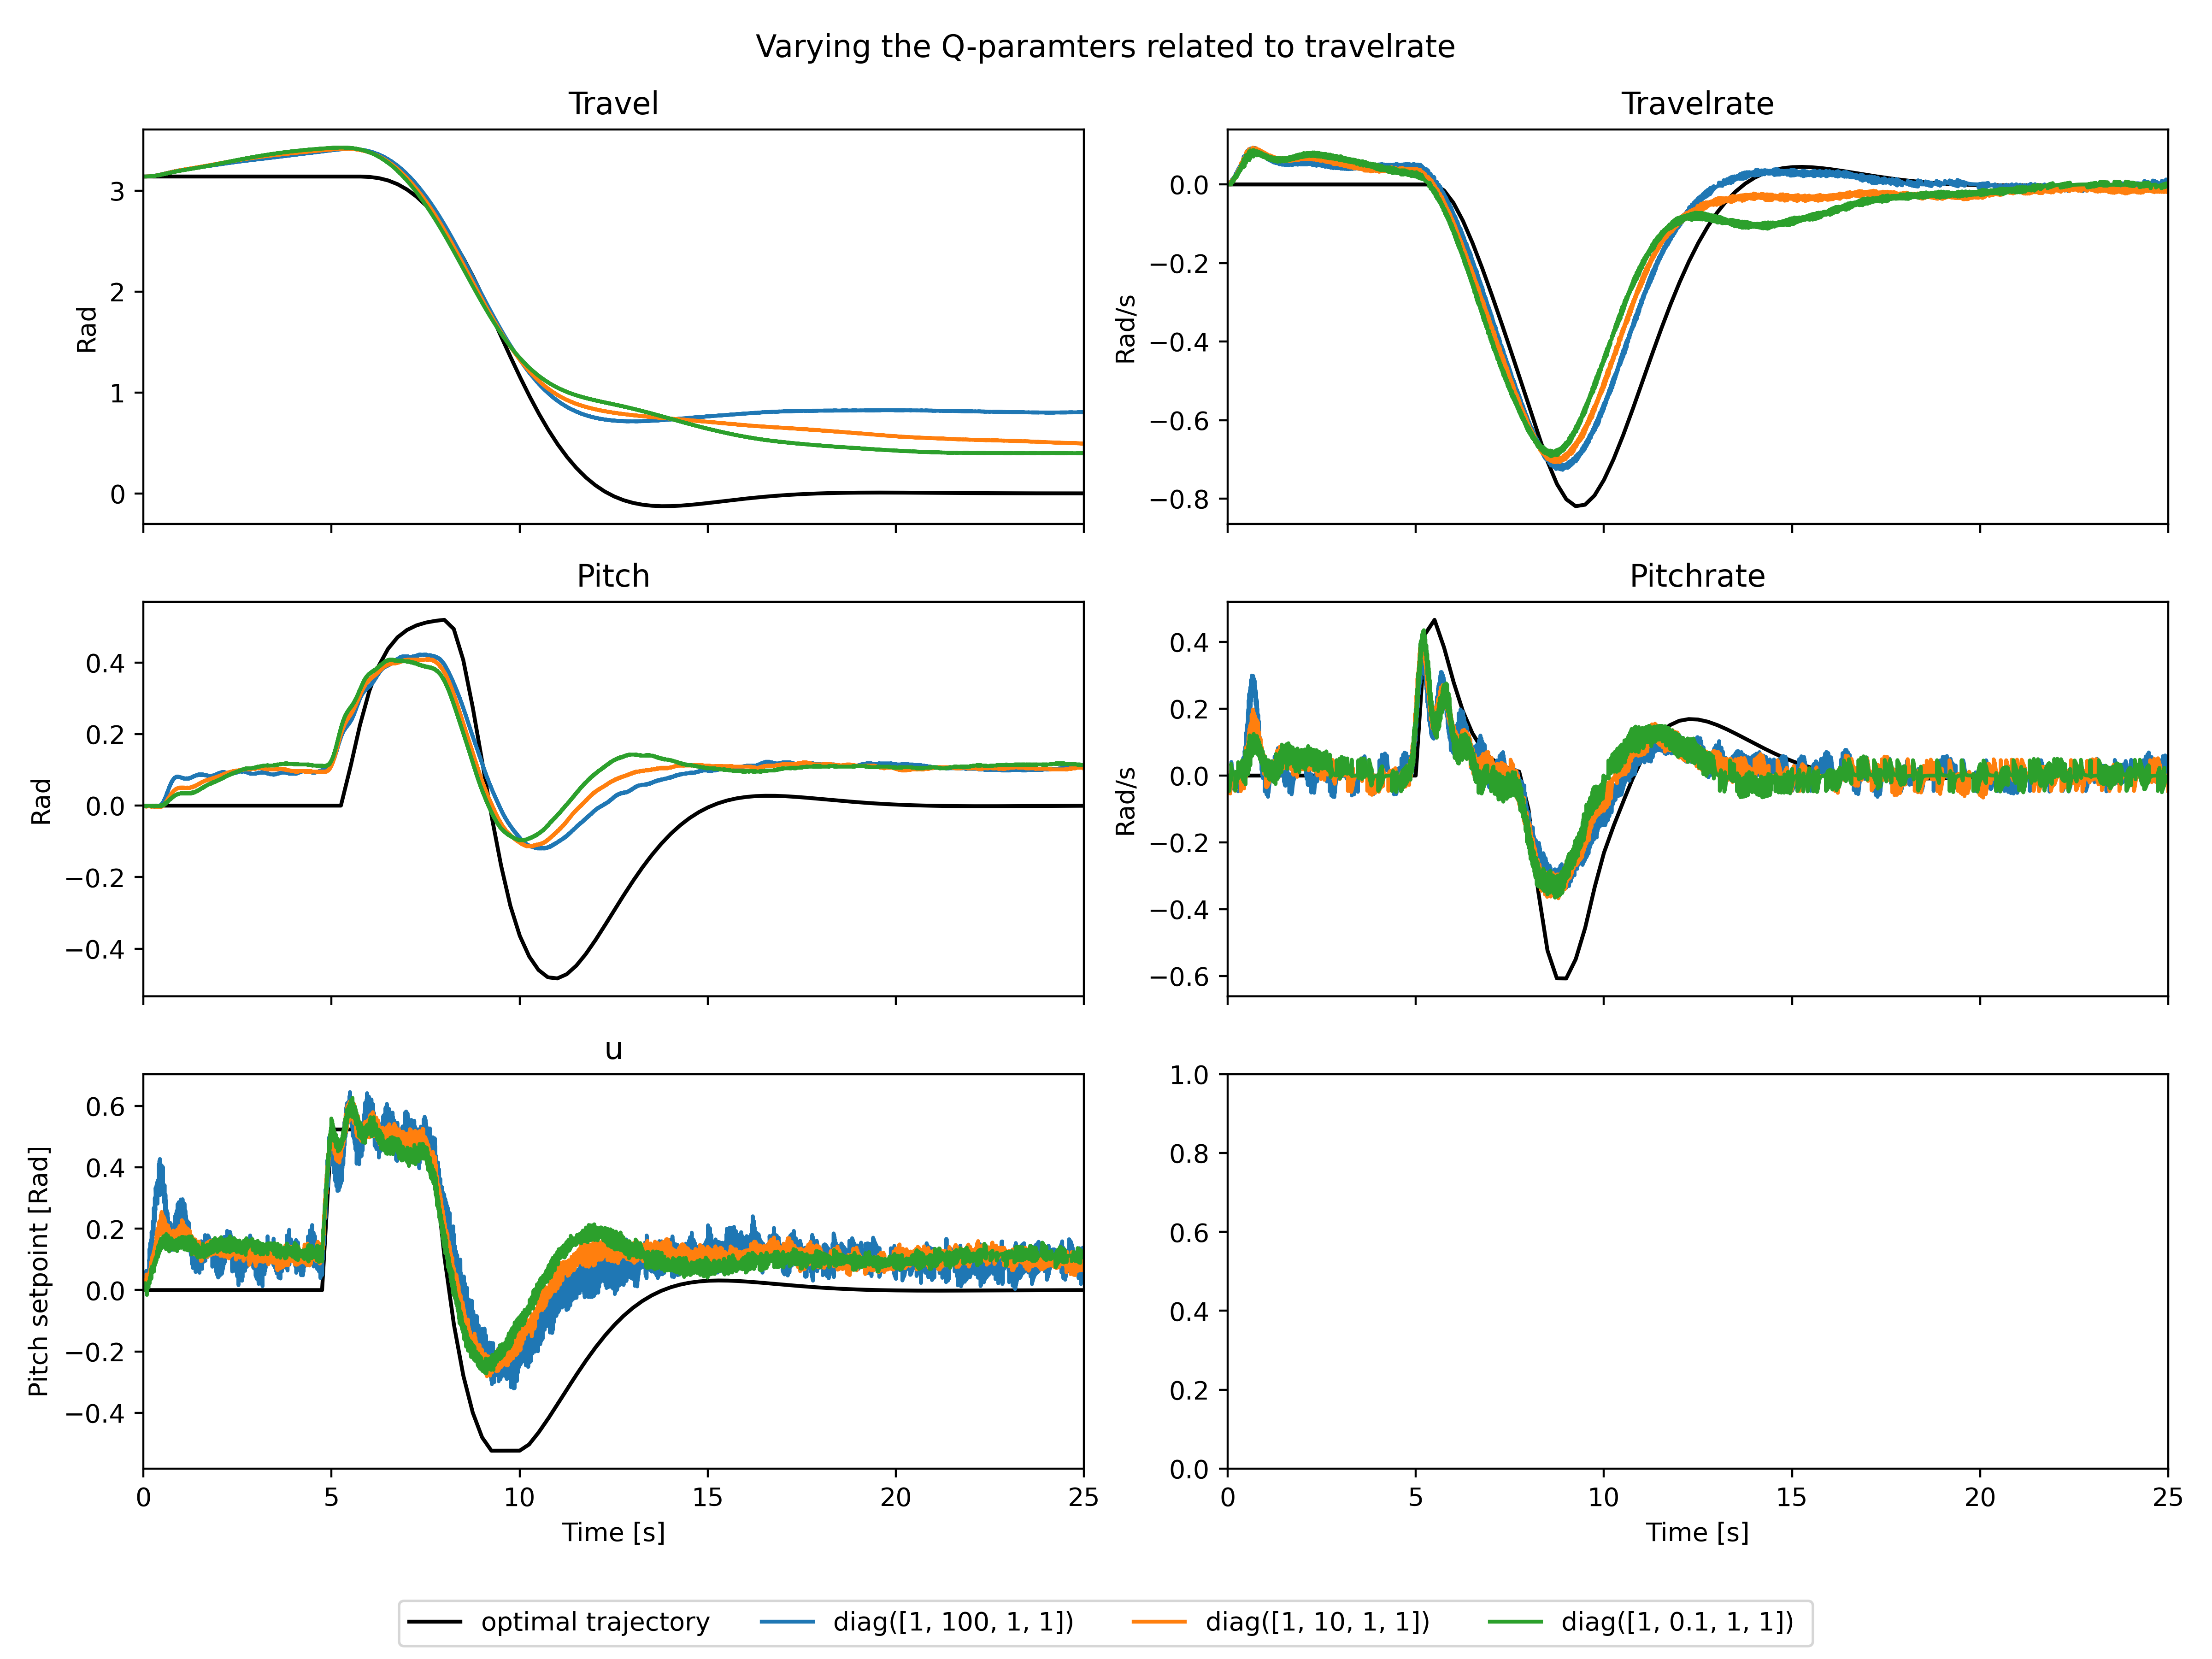
\includegraphics[width=\linewidth]{figures/LAB3_Q_variations_travelrate.png}
	\caption{Results of varying Q-values while keeping $R=1$}
	\label{fig:LAB3_Q_variations_travelrate}
\end{figure}

\begin{figure}[h]
	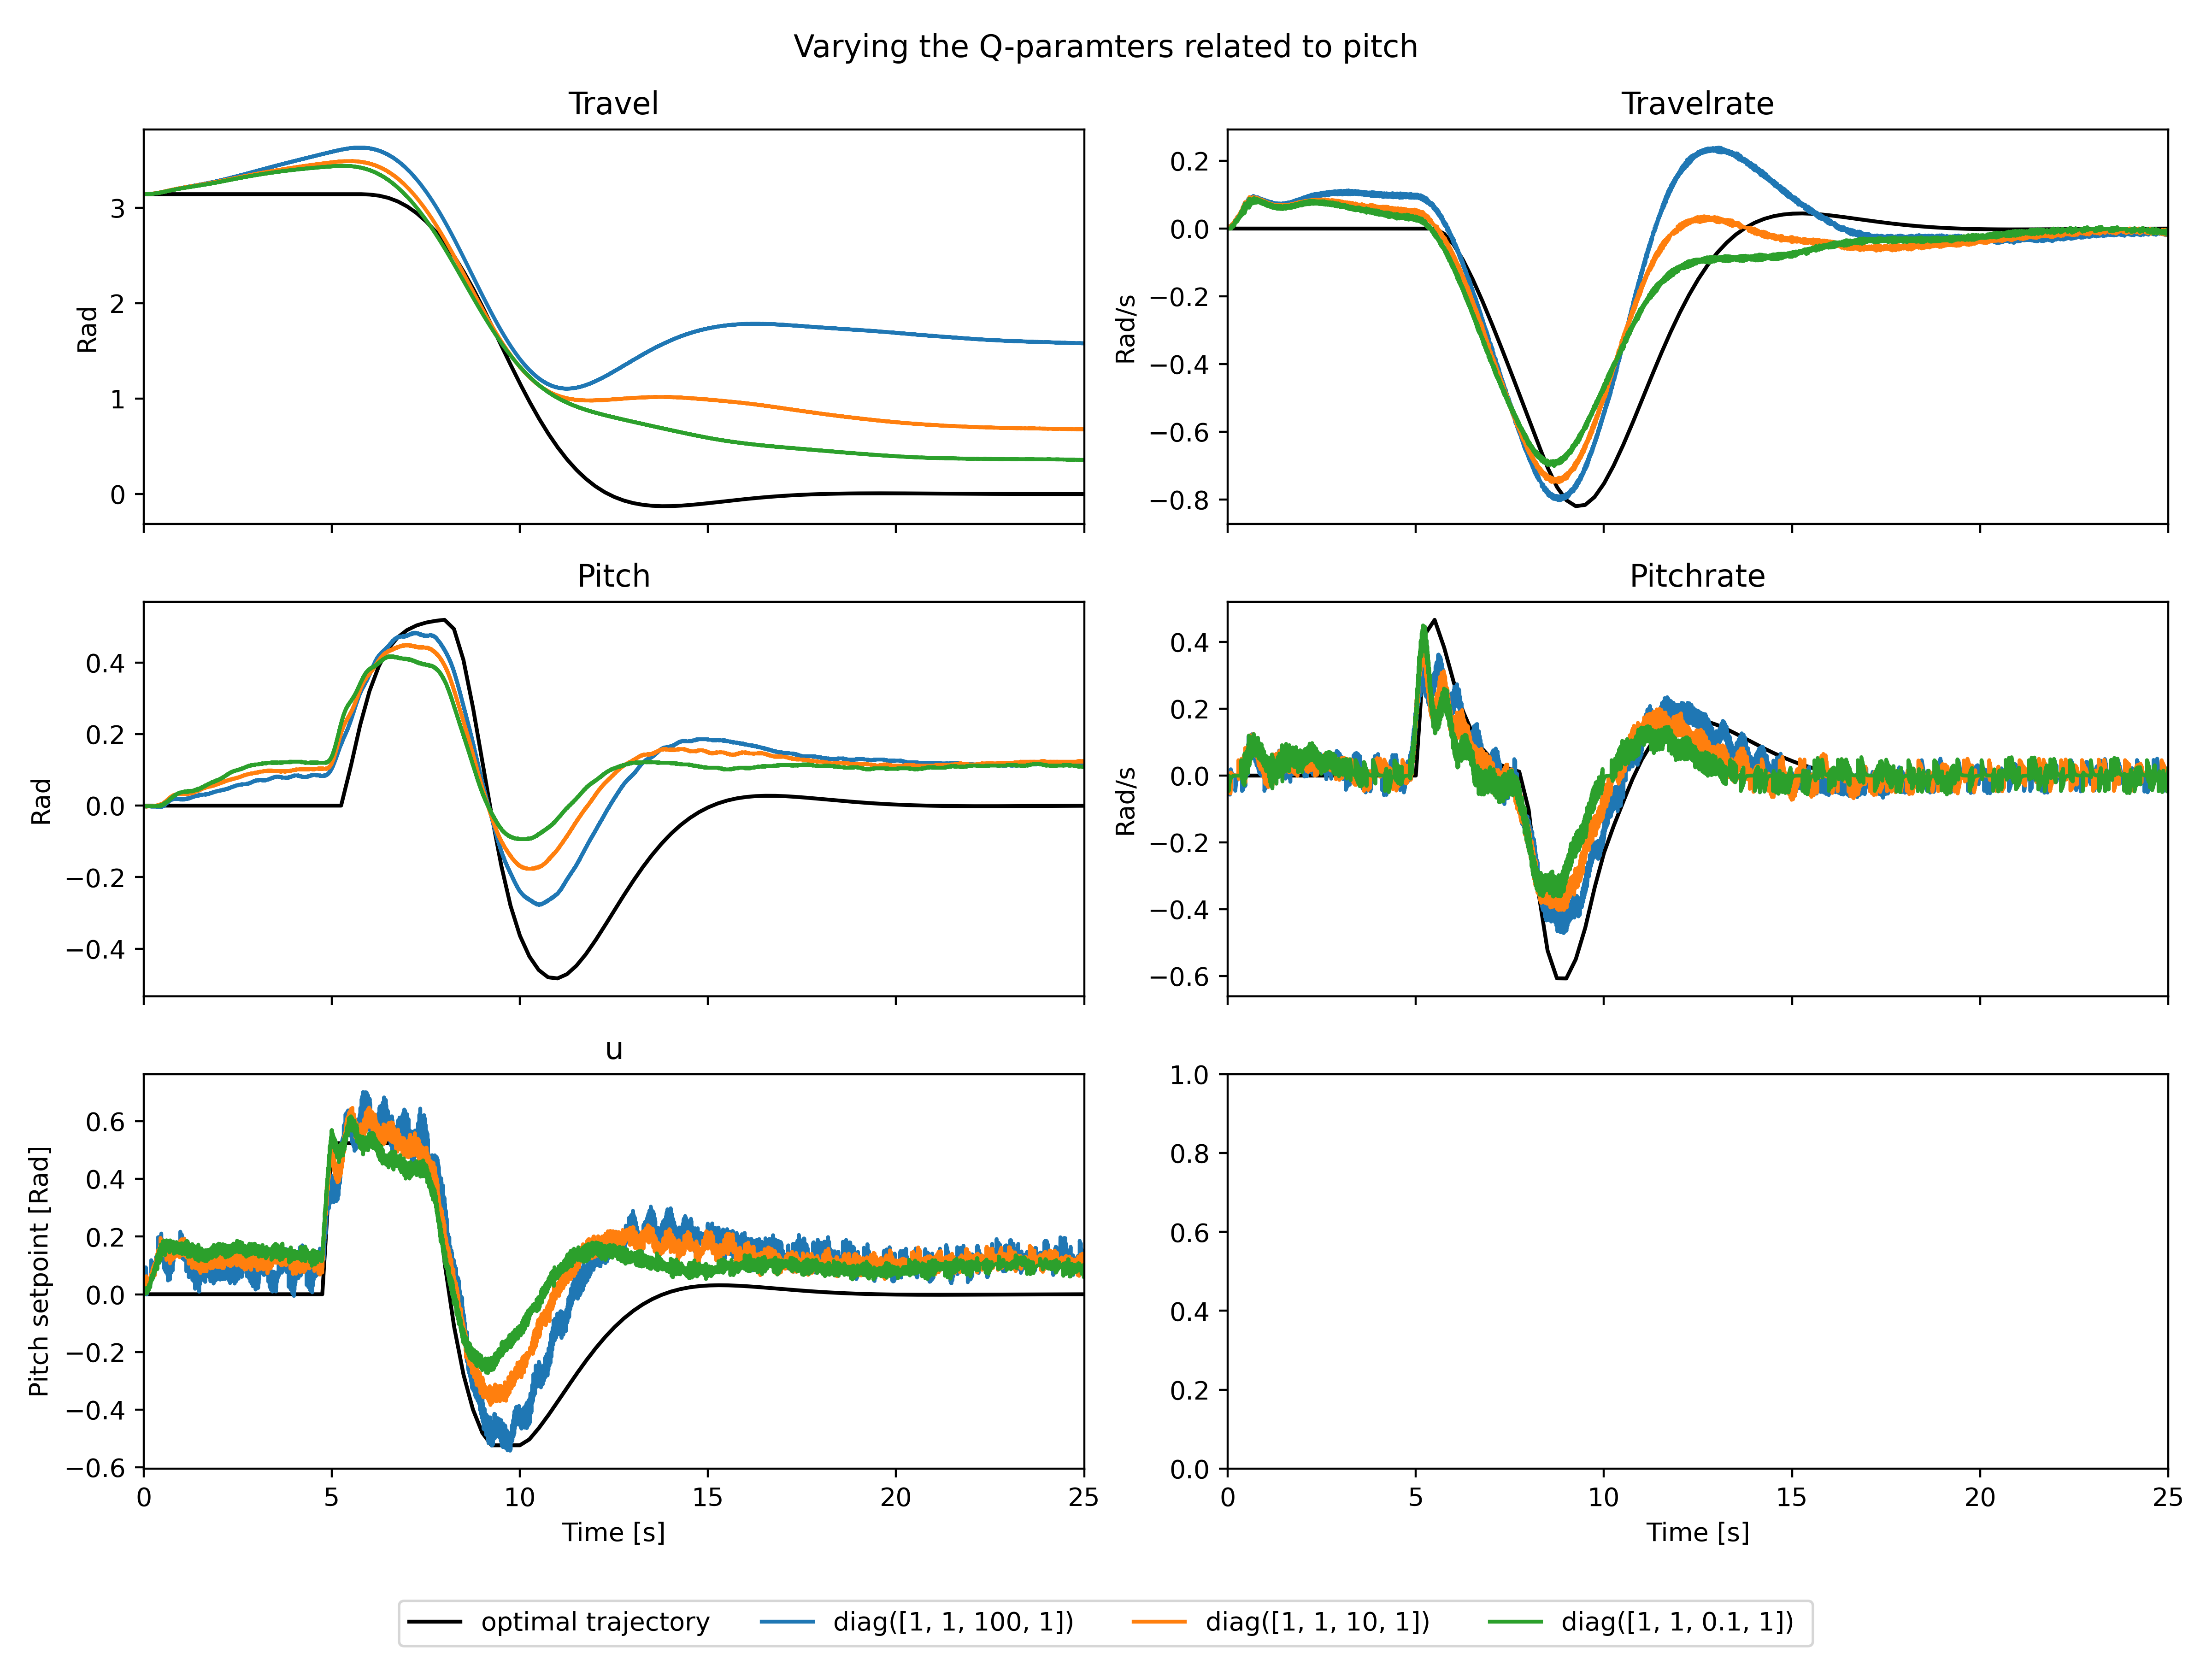
\includegraphics[width=\linewidth]{figures/LAB3_Q_variations_pitch.png}
	\caption{Results of varying Q-values while keeping $R=1$}
	\label{fig:LAB3_Q_variations_pitch}
\end{figure}

\begin{figure}[h]
	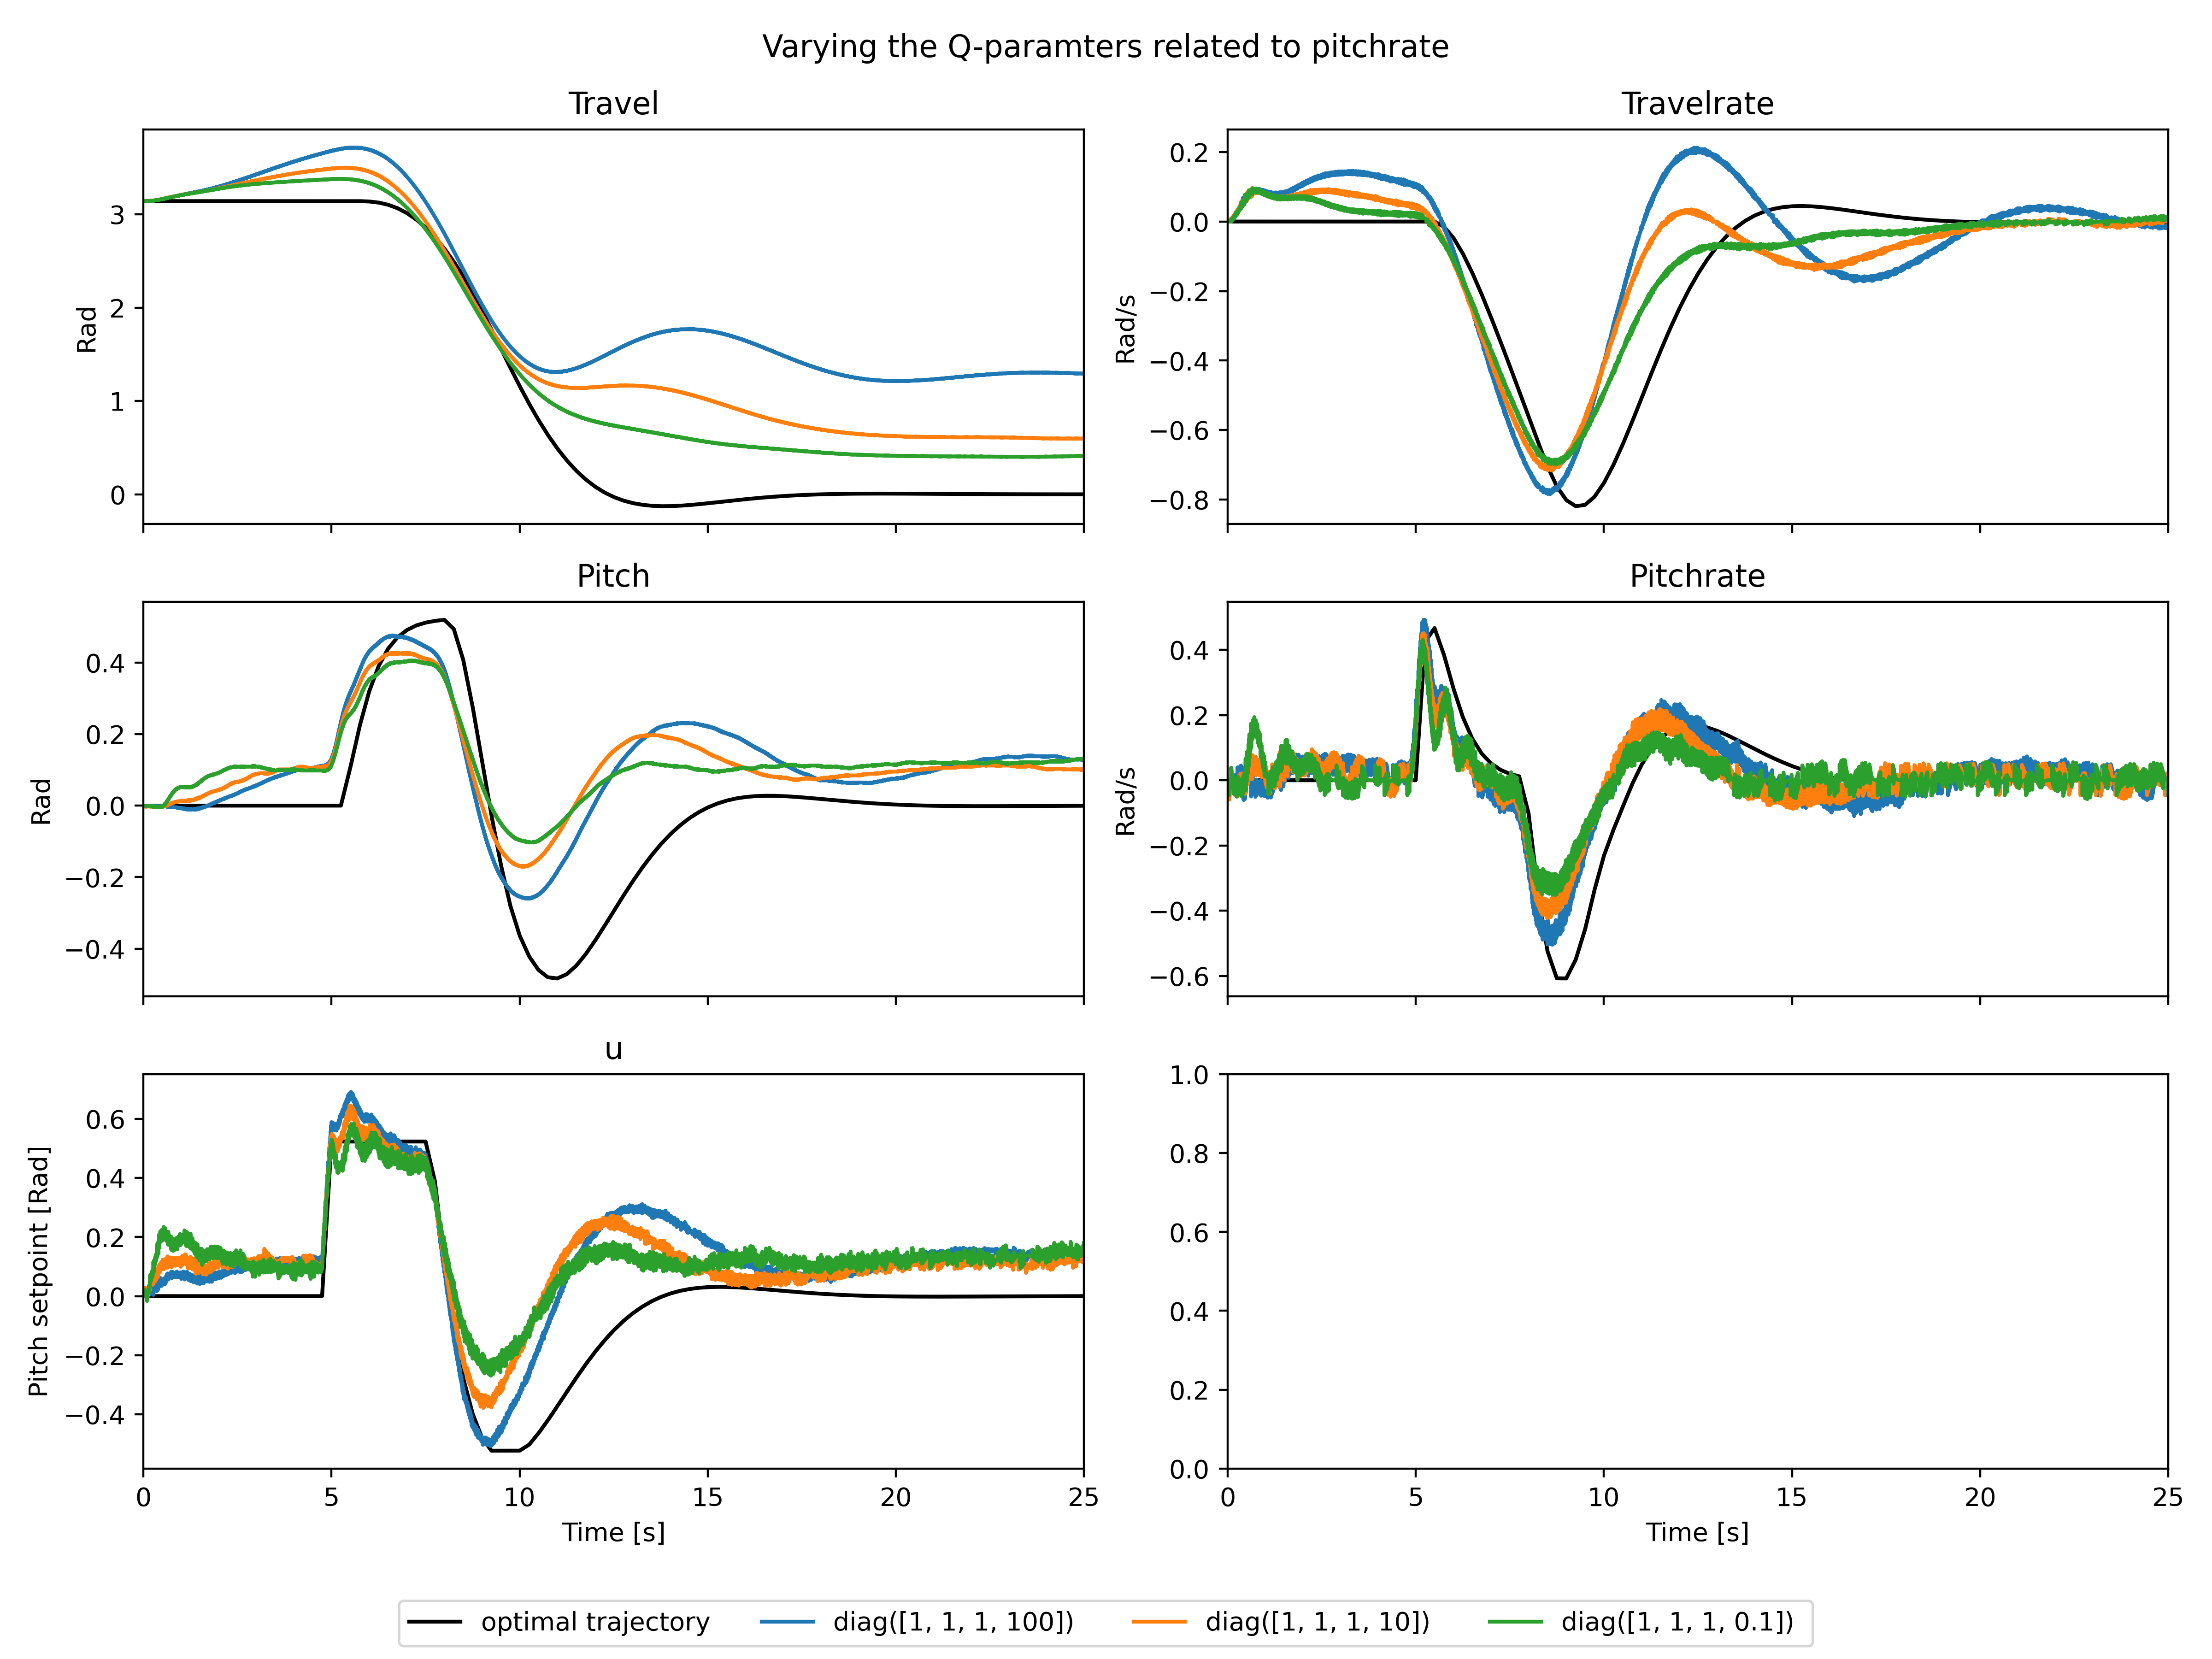
\includegraphics[width=\linewidth]{figures/LAB3_Q_variations_pitchrate.png}
	\caption{Results of varying Q-values while keeping $R=1$}
	\label{fig:LAB3_Q_variations_pitchrate}
\end{figure}


\clearpage

\subsection{MATLAB and Simulink}
\textit{Code and diagrams go here}
\end{document}